% !TEX encoding = UTF-8 Unicode

\documentclass[10pt,reqno]{amsart}
\usepackage[russian]{babel}
\usepackage[utf8]{inputenc}
\usepackage{geometry}
\geometry{verbose,a4paper,tmargin=2cm,bmargin=2cm,lmargin=2.5cm,rmargin=1.5cm}
%\usepackage[dvips]{graphicx,graphics}
\usepackage{graphicx}
\usepackage{euscript}
\usepackage{graphics}
\usepackage{centernot}
%\usepackage{russcorr}
\usepackage[active]{srcltx} % SRC Specials: DVI [Inverse] Search
\usepackage{amssymb,amsmath,amsthm,amsfonts}
\usepackage{amsopn}
\newtheorem{cor}{Следствие}
\newtheorem{lem}{Лемма}
\newtheorem{thm}{Теорема}
\newtheorem{prop}{Предложение}
\newtheorem*{thm_pres}{Теорема}
\theoremstyle{definition}
\newtheorem{defn}{Определение}
\newtheorem{defneq}{Эквивалентное определение}
\theoremstyle{remark}
\newtheorem*{rem}{Замечание}
\newtheorem*{deff}{Обозначение}
\newtheorem{ex}{Пример}
\usepackage{verbatim}
\usepackage{listings}
\usepackage{verbatim}
\usepackage{tabularx}
\usepackage{pbox}
\usepackage{bussproofs}

\newcommand{\lfrac} [2] {\displaystyle \frac{#1}{#2}}
\newcommand{\brsum} [3] {\displaystyle \sum \limits_{#1}^{#2} \left( #3\right)}
\newcommand{\lsum} [2] {\displaystyle \sum \limits_{#1}^{#2}}
\newcommand{\br} [1] {\left( #1 \right)}
\usepackage{a4wide}
\begin{document}
\section*{Задача 1.}

\subsection*{Метод Вальда:}


Статистика: $\widehat{p} \pm z_{1 - \frac{\alpha}{2}} \sqrt{\frac{\widehat{p}(1 - \widehat{p})}{n}}$

Особенности:
\begin{itemize}
\item Критерий Вальда ориентирует статистику на самые неблагоприятные условия.
\item Тест является асимптотическим, то есть для достоверности выводов требуется достаточно большой объём выборки.
\item Метод не рекомендуется при малых объемах выборок и в случаях, когда частота встречаемости признака стремится к 0 или 1
\item Может выходить за пределы [0,1]
\item При $\widehat{p}$ = 0 или 1 вырождается в точку
\item Накрывает $\widehat{p}$  реже чем $100(1 - a)\%$ случаев
\end{itemize}

Таким образом, несмотря на простоту расчетов, метод Вальда может применяться лишь в очень ограниченном числе случаев.


\subsection*{Метод Уилсона:}

Статистика: $\frac{T + z_{1 - \frac{\alpha}{2}} / 2}{n + z_{1 - \frac{\alpha}{2}}} \pm \frac{z_{1 - \frac{\alpha}{2}} \sqrt{n}}{n + z^2_{1 - \frac{\alpha}{2}}}\sqrt{\widehat{p}(1 - \widehat{p}) + \frac{z^2_{1 - \frac{\alpha}{2}}}{4n}}$


Особенности:
\begin{itemize}
\item Основан на критериии меток.
\item Плохо себя ведет при $\widehat{p}$ близком к 1 или 0
\item В среднем уровень довария равен номинальному
\item Применим для малого числа наблюдений
\end{itemize}


\subsection*{Метод Клоппера-Пирсона:}

Статистика: определяется квантилями бета-распределения

Особенности:
\begin{itemize}
\item Основан на биномиальном критерии
\item Уровень доверия никогда не ниже номинального
\item Доверительные интервалы, полученные таким образом, в большинстве случаев слишком широки
\item Степень консервативности метода увеличивается по мере уменьшения объема выборки
\end{itemize}

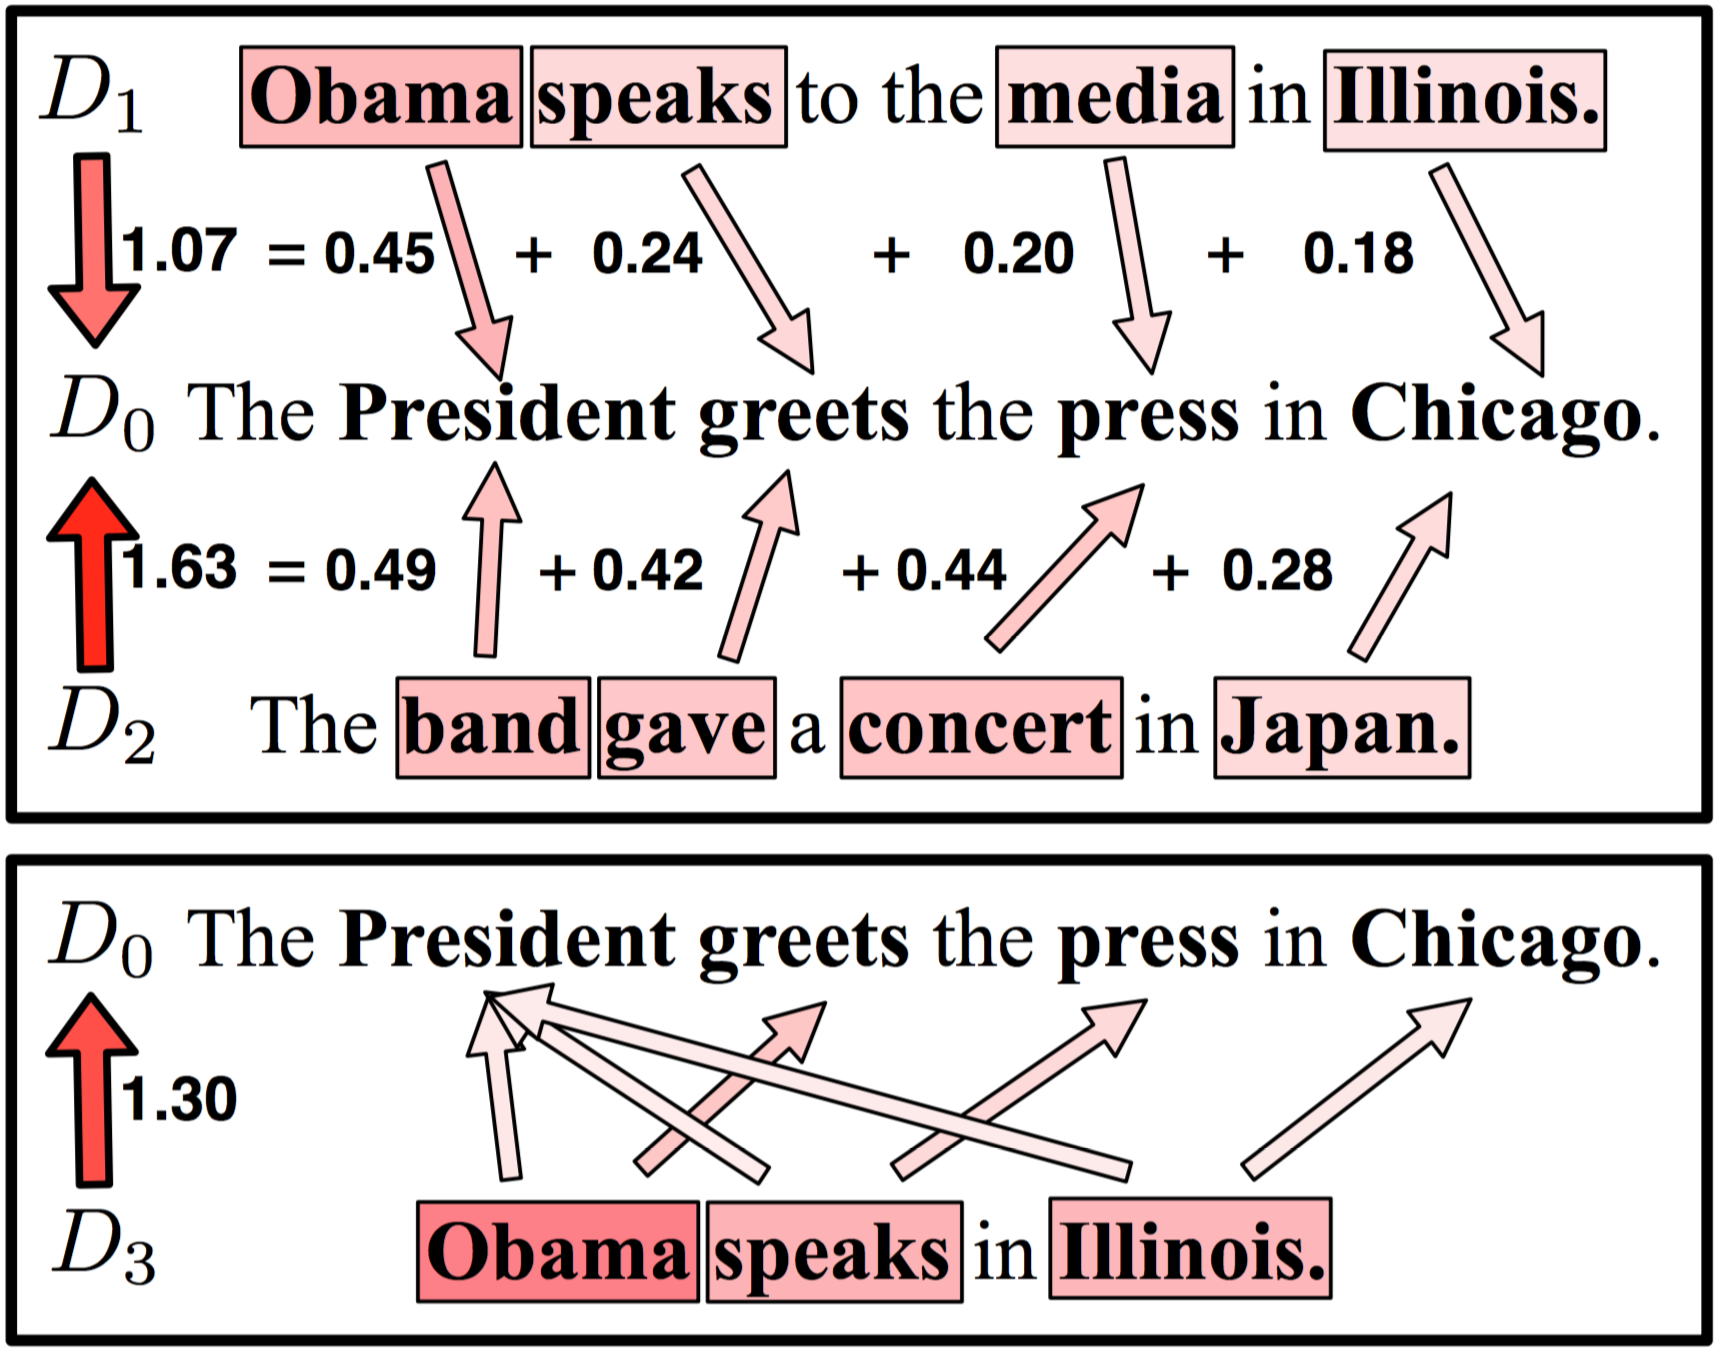
\includegraphics[scale=0.3]{1.png}


$>$ Клоппера-Пирсона
$>$ Вальд
$>$ Уилсон

\section*{Задача 2.}

Правые значения уползают слишком сильно вверх от нормальной линии это значит что максимальные значения нашего распределения слишком больши(высоки) для нормального

Слева точки выше нормальной линии -- значение не хватает сильно выраженных минимальных значений


Картинка...

\section*{Задача 3.}
\subsection*{a)}

Так как группы независимы то можно использовать Z-критерий для разности двух долей(независимые выборки):

\begin{tabular}{| l | c | r |}
        \hline
        * & X1 & X2 \\
        \hline
        1 & a & b \\
        \hline
        0 & c & d \\
        \hline
        $\sum$ & $n_1$ & $n_2$ \\
        \hline
\end{tabular}


Статистика: $Z(X_1, X_2) = \lfrac{\widehat{p_1} - \widehat{p_2}}{\sqrt{P(1 - P) \left( \frac{1}{n1} + \frac{1}{n2}\right)}}$

Где: $P = \lfrac{\widehat{p_1}n_1 - \widehat{p_2}n_2}{n_1 + n_2}$, $\widehat{p_1} = \lfrac{a}{n1}$, $\widehat{p_2} = \lfrac{b}{n2}$

Нулевое распределение: $N(0,1)$

\subsection*{б)}
Группы стали зависимыми так как состоят из одних и тех же людей в обоих опытах поэтмоу надо и Z-критерий для разности двух долей, связанные выборки

\begin{tabular}{| l | c | r |}
	\hline
	* & X1 & X2 \\
	\hline
	1 & e & f \\
	\hline
	0 & g & h \\
	\hline
\end{tabular}

Статистика: $Z(X_1, X_2) = \lfrac{\widehat{p_1} - \widehat{p_2}}{\sqrt{\frac{f + g}{n^2} + \frac{(f - g)^2}{n^3}}}$

Нулевое распределение: $N(0,1)$

Учитываются только те элементы на которых значение поменялось. По этому критерию интервал получится уже.

Для связных выборок критерий использует больше информаци, следовательно он мощнее.


\section*{Задача 4.}

Благодаря центральной предельной теореме и удобству вывода критериев для нормально распределённых выборок методы, основанные на предположении о нормальности данных, наиболее широко распространены. Если принять предположение о нормальности, то можно применять более мощные критерии. Зачастую они также чувствительны к небольшим отклонениям от нормальности. Если гипотеза нормальности отвергается, следует использовать не параметрические методы.

\subsection*{Критерий согласия Пирсона}
Основан на сравнении эмпирических частот интервалов группировки с теоретическими (ожидаемыми) частотами, рассчитываемыми по формулам нормального распределения

Cтатистика: $\chi^2(X^n) = \sum_{i = 1}^{K} \lfrac{(n_i - np_i)^2}{npi}$


Где: $[a_i, a_{i+1}], i=1,...,K$ -- интервалы гистограммы, $n_i$ -- число элементов выборки лежащих в $[a_i, a_{i+1}]$, $p_i = F(a_{i + 1}) - F(a_i)$ - вероятность попадания в i-й интервал при $H_0$.


Нулевое распределение: если $\mu, \sigma$ оценены то $\chi^2_{K-3}$, иначе $\chi^2_{K-1}$


Недостатки:
\begin{itemize}
\item Разбиение на интервалы никак не фиксированно --> выбирая разные интервалы можно получать разные результаты
\item Требует больших выборок ($np_i > 5$ в $80\%$ интервалах)
\end{itemize}


\subsection*{Критерий Колмогорова.}

Предназначен для проверки гипотезы о принадлежности выборки некоторому закону распределения, то есть проверки того, что эмпирическое распределение соответствует предполагаемой модели.

Cтатистика: $D(X_n) = \sup_{-\infty < x < \infty} |F_n(x) - \Phi(x)|$

Нулевое распределение: табличное

Недостатки:
\begin{itemize}
\item Имеет низкую мощность
\item Не чувствителен к различиям на хвостах распределений
\end{itemize}

\subsection*{Критерий Шапиро Уилка}
Основан на отношении оптимальной линейной несмещенной оценке дисперсии к ее обычной оценке методом максимального правдоподобия(Основан на анализе qq графика)
Один из наиболее эффективных критериев


Cтатистика: $W(X_n) = \lfrac{\left(\sum_1^n a_i X_{(i)}\right)^2}{\sum_1^n (X_i - \overline{X})^2}$

Где: $(a_1,...,a_n) = \lfrac{m^TV^{-1}}{m^TV^{-1}V^{-1}m}$, $m = (m_1,...,m_n)^T$ -- матожидания порядковых статистик $N(0, 1)$, V — их ковариационная матрица;

Нулевое распределение: табличное

Недостатки: для больших n таблицы коэффициентов становятся неудобным

\section*{Задача 5.}
4. Z-критерий

5. t-критерий Стьюдента / Аспина-Уэлша (проблема Беренца-Фишера)

6. t-критерий Стьюдента для связанных выборок

7. F-критерий Фишера
\end{document}
